%%!TEX TS-program = latex
\documentclass[]{beamer}
%\usepackage{helvet}
%\usepackage{pstricks,pst-node,pst-tree}
\usepackage{graphicx}
\hypersetup{pdfpagemode=FullScreen}
\usetheme{Singapore}
%\usetheme{copenhagen}
%\usetheme{Boadilla}
%\usetheme{Warsaw} 
\usecolortheme{seagull} 
\setbeamercovered{transparent}
\beamertemplatenavigationsymbolsempty 
\setbeamertemplate{footline}[frame number]

\usepackage{hyperref}
\usepackage{amsmath}
\usepackage{amsfonts}
\usepackage{amssymb}
\usepackage{booktabs}
\usepackage{dsfont}
\usepackage{multicol}
\usepackage{multirow}

\newcommand{\R}{\ensuremath{\mathds{R}}}
\newcommand{\C}{\ensuremath{\mathds{C}}}
\newcommand{\Q}{\ensuremath{\mathds{Q}}}
\newcommand{\N}{\ensuremath{\mathcal{N}}}
\newcommand{\Z}{\ensuremath{\mathds{Z}}}

\setbeamerfont{bib}{size*={4.00}{4.00}}
\usepackage[square, sort, numbers, authoryear]{natbib}
\renewcommand{\bibsection}{\subsubsection*{\bibname } }


\DeclareMathOperator*{\argmax}{argmax}
\DeclareMathOperator*{\argmin}{argmin}
\DeclareMathOperator*{\Corr}{Corr}
\DeclareMathOperator*{\E}{E}
\DeclareMathOperator*{\sign}{sign}
\renewcommand{\vec}[1]{\mathbf{#1}}
\usepackage{hyperref}

\usepackage{multicol}
\usepackage{multirow}
\usepackage{pbox}


\institute[]{}
%\logo{\pgfimage[width=.8cm,height=.8cm]{../KU_logo}}
\title[Active Manifesto]{
{
Speeding up the Manifesto Project: \\ Active learning strategies for \\efficient automated political annotations
}}
\author{
Felix Biessmann\thanks{felix.biessmann@gmail.com},~ 
Philipp Schmidt\thanks{schmidtiphil@gmail.com}
}
\date{}
\begin{document}

\begin{frame} 
\titlepage 
\end{frame}	

%
\section{Intro}
\subsection{}

\begin{frame}\frametitle{Disclaimers}
\small
\begin{itemize}[<+->]
\item (For us) This is just a hobby / open source project
\item It has nothing to do with our job
\end{itemize}
\end{frame}

\begin{frame}\frametitle{Motivation}
\begin{itemize}[<+->]
\item Everyday loads of political content is published
\item Too much text to handle by humans
\item[$\rightarrow$] Automated political bias prediction\footnote{\cite{Biessmann16, Merz2016}} required for 
\begin{itemize}
\item Political scientists
\item Journalists
\item Average media consumer
\end{itemize}
\end{itemize}
\end{frame}

\begin{frame}\frametitle{Motivation}
\begin{itemize}[<+->]
\item Machine Learning models need fresh training data
\item But annotation budget is often limited:
\begin{itemize}
\item Temporal constraints (before elections) \cite{merz2017}
\item Online news media (too much content) 
\end{itemize}
\item[$\rightarrow$] How to select which texts to annotate?
\end{itemize}
\end{frame}

\begin{frame}\frametitle{Active Learning}
\begin{itemize}[<+->]
\item Train best model with limited budget
\item Annotate difficult ones\footnote{For which model is most uncertain.} first
\item Why?
\begin{itemize}
\item Intuition: \\
\textit{ Model learns most from difficult examples}\\
\item Math:\\
\textit{ Gradient of loss function larger for difficult examples }\\
\end{itemize}
\end{itemize}
\end{frame}

\section{Methods}
\subsection{}

\begin{frame}\frametitle{Data}
\begin{itemize}
\item All annotated German texts from \url{https://manifestoproject.wzb.eu/} 
\item Only texts with more than 1000 observed labels
\end{itemize}
\end{frame}

\begin{frame}\frametitle{Preprocessing}
\begin{itemize}
\item Basic text cleaning (regexps, stopwords)
\item Unigram Bag-of-Words features
\item Hashing Vectorizer
\end{itemize}
\end{frame}

\begin{frame}\frametitle{Classification Model: Multinomial Logistic Regression}
Manifestocode prediction is modelled as
\begin{eqnarray}\label{eq:logreg_multiclass}
p(y=k|\vec{x}) = \frac{e^{z_k}}{\sum_{j=1}^K e^{z_j}}  \textrm{ with }  z_k=\vec{w}_k^{\top}\vec{x}.
\end{eqnarray}
With
\begin{itemize}
\item Labels $y\in\{1,2,\dots,K\}$ (manifesto code)\\ 
\item $\vec{w}_1,\dots,\vec{w}_K\in\R^{d}$ weight vectors of $k$th manifesto code\\ 
\item $L_2$ norm regularization of weights
\end{itemize}
\end{frame}

\begin{frame}\frametitle{Active Learning Strategies}

\begin{itemize}
\item Random Baseline: Uniform random sampling
\item Uncertainty Sampling: Only top-prediction counts
\begin{align}\label{eq:uncertainty_sampling}
\vec{x}_i = \argmax_{i,k} \left(1- p(y=k|\vec{x}_i,\vec{W})\right)
\end{align}
\item Entropy Sampling: All predictions count
\begin{align}\label{eq:entropy_sampling}
\vec{x}_i = \argmax_{i} \sum_k p(y=k|\vec{x}_i,\vec{W}) \log(p(y=k|\vec{x}_i,\vec{W}))
\end{align}
\item Margin Sampling: Top 2 predictions count
\begin{align}\label{eq:entropy_sampling}
\vec{x}_i = \argmin_{i} \left(p(y=k_1|\vec{x}_i,\vec{W}) - p(y=k_2|\vec{x}_i,\vec{W}) \right)
\end{align}
\end{itemize}
\end{frame}

\begin{frame}\frametitle{Active Learning Experiments}

\begin{itemize}
\item Train model on 1\%, 10\%, 20\%, \dots, 100\% of training data
\item Vary sampling strategies to select from unlabelled texts
\item Evaluate agains 'perfect' model trained on all data
\end{itemize}
\end{frame}


\section{Results}
\subsection{}


\begin{frame}\frametitle{Results: 'Perfect' Reference Model}
\footnotesize
\begin{table}
\centering
\begin{tabular}{cccccc}
\toprule
&  manifesto code & precision  &  recall&  f1-score &  support\\
\midrule
&   107&  0.60& 0.48& 0.53&  774\\
&   201&  0.51& 0.55& 0.53& 1194\\
&   202&  0.63& 0.57& 0.60&  983\\
&   305&  0.46& 0.59& 0.52&  783\\
&   403&  0.52& 0.48& 0.50& 1281\\
&   411&  0.39& 0.60& 0.47& 1535\\
&   501&  0.61& 0.55& 0.58& 1380\\
&   502&  0.65& 0.41& 0.50&  587\\
&   503&  0.46& 0.52& 0.49& 2083\\
&   506&  0.63& 0.48& 0.54& 1026\\
&   605&  0.56& 0.44& 0.49&  576\\
&   701&  0.59& 0.39& 0.47& 1123\\
\bottomrule
& avg / total&  0.50& 0.48& 0.48&17559\\
\end{tabular}
\caption{Precision, recall, F1 score and number of instances per class. }
\label{tab:baseline_model_report} 
\end{table}

\end{frame}

\begin{frame}\frametitle{Active Learning Results}
\begin{center}
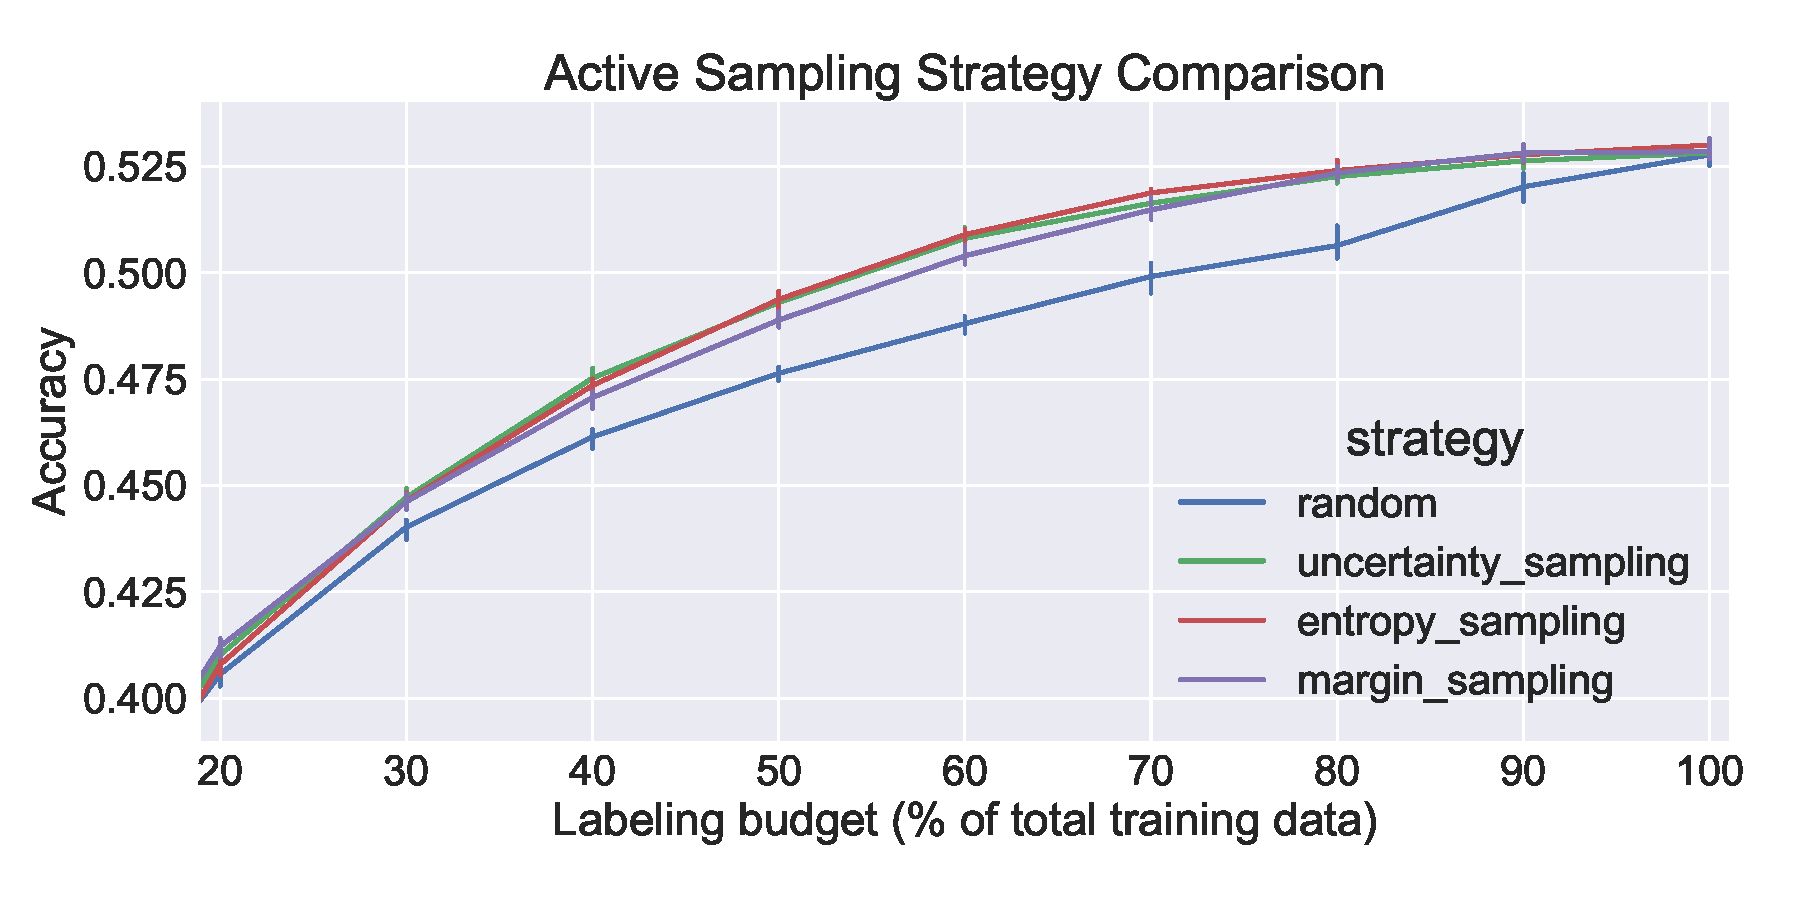
\includegraphics[width=\textwidth]{images/active_learning_manifesto.pdf} \\
Median accuracy and the 5th/95th percentile across 100 repetitions \\
\end{center}

\end{frame}

\section{Conclusion}
\subsection{}


\begin{frame}\frametitle{Conclusion}
\begin{itemize}
\item Political text analysis requires automation
\item Automation requires annotations for training models
\item Limited budged for annotations of political texts 
\item Active Learning
\begin{itemize}
\item Helps to select which texts to annotate
\item Perfect model with 80\% of data
\item Almost perfect (over 95\%) with 50\% of data
\end{itemize}
\item[$\rightarrow$] Active learning can speed up political annotations. 
\item Demo: \url{http://rightornot.info}
\end{itemize}
\end{frame}

\begin{frame}\frametitle{References}
\usebeamerfont{bib}

\bibliographystyle{abbrvnat}
\def\newblock{}
\vspace{2em}
\bibliography{active-manifesto} 
\end{frame}

\end{document} 
